% Version 1.2 of SN LaTeX, November 2022
%
% See section 11 of the User Manual for version history 
%
%%%%%%%%%%%%%%%%%%%%%%%%%%%%%%%%%%%%%%%%%%%%%%%%%%%%%%%%%%%%%%%%%%%%%%
%%                                                                 %%
%% Please do not use \input{...} to include other tex files.       %%
%% Submit your LaTeX manuscript as one .tex document.              %%
%%                                                                 %%
%% All additional figures and files should be attached             %%
%% separately and not embedded in the \TeX\ document itself.       %%
%%                                                                 %%
%%%%%%%%%%%%%%%%%%%%%%%%%%%%%%%%%%%%%%%%%%%%%%%%%%%%%%%%%%%%%%%%%%%%%

%%\documentclass[referee,sn-basic]{sn-jnl}% referee option is meant for double line spacing

%%=======================================================%%
%% to print line numbers in the margin use lineno option %%
%%=======================================================%%

%%\documentclass[lineno,sn-basic]{sn-jnl}% Basic Springer Nature Reference Style/Chemistry Reference Style

%%======================================================%%
%% to compile with pdflatex/xelatex use pdflatex option %%
%%======================================================%%

%%\documentclass[pdflatex,sn-basic]{sn-jnl}% Basic Springer Nature Reference Style/Chemistry Reference Style


%%Note: the following reference styles support Namedate and Numbered referencing. By default the style follows the most common style. To switch between the options you can add or remove “Numbered” in the optional parenthesis. 
%%The option is available for: sn-basic.bst, sn-vancouver.bst, sn-chicago.bst, sn-mathphys.bst. %  
 
%%\documentclass[sn-nature]{sn-jnl}% Style for submissions to Nature Portfolio journals
%%\documentclass[sn-basic]{sn-jnl}% Basic Springer Nature Reference Style/Chemistry Reference Style
\documentclass[sn-mathphys,Numbered]{sn-jnl}% Math and Physical Sciences Reference Style
%%\documentclass[sn-aps]{sn-jnl}% American Physical Society (APS) Reference Style
%%\documentclass[sn-vancouver,Numbered]{sn-jnl}% Vancouver Reference Style
%%\documentclass[sn-apa]{sn-jnl}% APA Reference Style 
%%\documentclass[sn-chicago]{sn-jnl}% Chicago-based Humanities Reference Style
%%\documentclass[default]{sn-jnl}% Default
%%\documentclass[default,iicol]{sn-jnl}% Default with double column layout

%%%% Standard Packages
%%<additional latex packages if required can be included here>

\usepackage[spanish]{babel}
\selectlanguage{spanish}

\usepackage{graphicx}%
\usepackage{multirow}%
\usepackage{amsmath,amssymb,amsfonts}%
\usepackage{amsthm}%
\usepackage{mathrsfs}%
\usepackage[title]{appendix}%
\usepackage{xcolor}%
\usepackage{textcomp}%
\usepackage{manyfoot}%
\usepackage{booktabs}%
\usepackage{algorithm}%
\usepackage{algorithmicx}%
\usepackage{algpseudocode}%
\usepackage{listings}%---->para redactar codigo

%%%%

\usepackage[spanish,onelanguage]{algorithm2e}
%%%%%=============================================================================%%%%
%%%%  Remarks: This template is provided to aid authors with the preparation
%%%%  of original research articles intended for submission to journals published 
%%%%  by Springer Nature. The guidance has been prepared in partnership with 
%%%%  production teams to conform to Springer Nature technical requirements. 
%%%%  Editorial and presentation requirements differ among journal portfolios and 
%%%%  research disciplines. You may find sections in this template are irrelevant 
%%%%  to your work and are empowered to omit any such section if allowed by the 
%%%%  journal you intend to submit to. The submission guidelines and policies 
%%%%  of the journal take precedence. A detailed User Manual is available in the 
%%%%  template package for technical guidance.
%%%%%=============================================================================%%%%

%\jyear{2021}%

%% as per the requirement new theorem styles can be included as shown below
\theoremstyle{thmstyleone}%
\newtheorem{theorem}{Theorem}%  meant for continuous numbers
%%\newtheorem{theorem}{Theorem}[section]% meant for sectionwise numbers
%% optional argument [theorem] produces theorem numbering sequence instead of independent numbers for Proposition
\newtheorem{proposition}[theorem]{Proposition}% 
%%\newtheorem{proposition}{Proposition}% to get separate numbers for theorem and proposition etc.

\theoremstyle{thmstyletwo}%
\newtheorem{example}{Example}%
\newtheorem{remark}{Remark}%

\theoremstyle{thmstylethree}%
\newtheorem{definition}{Definition}%

\raggedbottom
%%\unnumbered% uncomment this for unnumbered level heads

\begin{document}

\title[Article Title]{Análisis y Comportamiento Predictivo Mediante Aprendizaje Automático en Sondeos Eléctricos Verticales, Aplicación en Adquisición de Datos}

%%=============================================================%%
%% Prefix	-> \pfx{Dr}
%% GivenName	-> \fnm{Joergen W.}
%% Particle	-> \spfx{van der} -> surname prefix
%% FamilyName	-> \sur{Ploeg}
%% Suffix	-> \sfx{IV}
%% NatureName	-> \tanm{Poet Laureate} -> Title after name
%% Degrees	-> \dgr{MSc, PhD}
%% \author*[1,2]{\pfx{Dr} \fnm{Joergen W.} \spfx{van der} \sur{Ploeg} \sfx{IV} \tanm{Poet Laureate} 
%%                 \dgr{MSc, PhD}}\email{iauthor@gmail.com}
%%=============================================================%%

\author*[1]{\pfx{Ing} \fnm{Torres S.} \sur{Juan J.}}\email{juan.j.torres.s@gmail.com}


\affil*[1]{\orgdiv{Facultad de Ciencias Físico Matemáticas}, \orgname{Maestr\'ia Ciencia de Datos}, \orgaddress{\street{Pedro de Alba, Niños Héroes}, \city{San Nicolás de los Garza}, \postcode{66451}, \state{N.L.}, \country{México}}}


%%==================================%%
%% sample for unstructured abstract %%
%%==================================%%

%\abstract{Aplicando metodolog\'ias de Aprendizaje Autom\'atico se realiza el entrenamiento de algoritmos, buscando generar el reconocimiento temprano de anomal\'ias en mediciones de Resistividad Aparente, en ensayos de Sondeos El\'ectricos verticales, cuyo tendencia y comportamiento se relaciona a zonas de saturaci\'on en el subsuelo, los datos se componen de los siguientes, sondeos de control y aleatorios a fin de generar un reconocimiento en distintos contrastes, aplicando XXXXXX y obteniendo XXXXXX, como resultado se puede observar un claro/nula respuesta en predicciones de acu\'ifero, teniendo un porcentaje  \% error , \% exito,... }

%%================================%%
%% Sample for structured abstract %%
%%================================%%

\abstract{\textbf{Propósito:} Durante el proceso de adquisición de datos geoléctricos, se pueden presentar anomalías, ya sean errores de medición, error de muestreo, ruido ambiental, efectos de sitio, etc.., esta publicación tiene por finalidad generar un algoritmo de Aprendizaje Automático que permita identificar error en etapas tempranas de adquisición así como una pre-interpretación de unidades saturadas, con la finalidad de reducir las incertidumbre, mejorando la calidad de los datos y dar la oportunidad al aperador de corregirlos al momento, así como generar una alerta temprana de unidades saturadas con el objetivo de ampliar la resolución de la unidad en cuestión con el objeto de obtener mayor detalle de estas zonas de interés.
% 
 \textbf{Método:} para lograr el propósito se empleara un conjunto de 647 datos, correspondientes a 29 Sondeos Eléctricos Verticales (SEV), realizados a lo largo de un año de mediciones, en configuraciones geológicas completamente distintas.
% 
% \textbf{Results:} The abstract serves both as a general introduction to the topic and as a brief, non-technical summary of the main results and their implications. The abstract must not include subheadings (unless expressly permitted in the journal's Instructions to Authors), equations or citations. As a guide the abstract should not exceed 200 words. Most journals do not set a hard limit however authors are advised to check the author instructions for the journal they are submitting to.
% 
% \textbf{Conclusion:} The abstract serves both as a general introduction to the topic and as a brief, non-technical summary of the main results and their implications. The abstract must not include subheadings (unless expressly permitted in the journal's Instructions to Authors), equations or citations. As a guide the abstract should not exceed 200 words. Most journals do not set a hard limit however authors are advised to check the author instructions for the journal they are submitting to.
}

\keywords{Resistividad Aparente, Keyword2, Keyword3, Keyword4}

%%\pacs[JEL Classification]{D8, H51}

%%\pacs[MSC Classification]{35A01, 65L10, 65L12, 65L20, 65L70}

\maketitle

\section{Introducci\'on}\label{sec1}

En una campaña de exploración geofísica enfocada en recursos geohídricas se pueden emplear distintos métodos para determinar la existencia, profundidad y distribución del nivel freático de un acuífero, como son método de refracción sísmica, GPR (Ground Penetrating Radar) y métodos geoeléctricos, en este trabajo nos enfocaremos en la aplicación del método geoeléctrico en la modalidad de Sondeo Eléctrico Vertical, aplicando técnicas de AA en la adquisición geoeléctrica con un Resistivímetro Analógico, el método consiste en inducir una corriente eléctrica en el subsuelo a través de dos electrodos afianzados al terreno, al mismo tiempo se realiza la lectura del potencial inducido por el flujo de la corriente en otro par de electrodos, colocados a una distancia previamente definida, empleando la configuración eléctrica Schlumberger (Referencia año), obteniendo valores de resistividad aparente en cada sondeo, durante la adquisición de datos se recopila la siguiente información: 

\begin{itemize} 
	\item  Sitio de estudio representado por la clave asignada, numero de sondeo, sitio y localidad o solicitante.
	\item  Personal técnico que realizo el levantamiento de los datos
	\item  Fecha del estudio
	\item  Zona datum UTM
	\item  Coordenada Este 
	\item  Coordenada Norte
	\item  Altitud 
	\item  Profundidad de muestreo
	\item  K factor geométrico de arreglo Schlumberger
	\item  Distancia Media entre los Electrodos A y B 
	\item  Distancia entre los electrodos A y B
	\item  Distancia Media entre los electrodos M y N
	\item  La quinta parte de la Distancia entre los Electrodos M y N
	\item  Distancia entre los Electrodos M y N
	\item  Potencia Natural 1
	\item  Potencial Inducido 1
	\item  Corriente Inyectada 1
	\item  Potencia Natural 2
	\item  Potencial Inducido 2
	\item  Corriente Inyectada 2
	\item  Potencia Natural 3
	\item  Potencial Inducido 3
	\item  Corriente Inyectada 3
	\item  Media del Potencial Natural
	\item  Media Potencial Inducido
	\item  Media de las Diferencias entre Potencial Inducido y Potencial Natural
	\item  Media de la Corriente Inyectada
	\item  Resistividad eléctrica aparente 1
	\item  Resistividad eléctrica aparente 2
	\item  Resistividad eléctrica aparente 3
	\item  Media de las resistividad eléctrica 1 2 y 3
	\item  Resistividad Eléctrica Aparente Final
\end{itemize}

Normalmente la adquisición de datos, con equipos analógicos, es realizada por personal con experiencia, sin embargo este no siempre es el caso, por lo que es resulta conveniente tener herramientas que nos permitan tener la oportunidad de mejor la calidad de los datos con alertas tempranas durante el registro de la adquisición geofísica, reduciendo los errores de muestreo y atenuando la incertidumbre de datos adquiridos por un operador inexperto.

\section{Marco Teórico}\label{sec2}

\subsection{Modelo No Supervisado}\label{subsec1}

\subsection{Modelo Supervisado: Isolation Forest}\label{subsec2}


\section{Metodología}\label{sec3}
Para este proyecto se trabajaran con datos de Resistividad eléctrica, adquiridos durante campañas de exploración en distintas zonas de México, sumando un total de 647 registros correspondientes a 29 sondeos, por protección de los clientes se cambiaron nombres de personal y ubicaciones geográfica, cambiando la ubicación de los sitios por un cuadrante del municipio San Nicolás de los Garza ubicado en el Estado de Nuevo León, para fines prácticos.

Se aplicaron métodos estadísticos descriptivos básicos, correlación entre variables y entrenamientos de modelos supervisados y no supervisados; en cada paso del proceso se genero información que permitió avanzar en el objetivo del estudio así como otorgar un panorama de lo general a lo particular a fin de alcázar el modelado predictivo.

\subsection{Reorganización y Preparación De Los Datos}\label{subsec3}

En esta etapa del trajo se procedió a reagrupar las columnas, descartando aquellas que no se relacionan directamente con el objetivo del trabajo, posteriormente se procese a eliminar las columnas que no contienen información o que presentan valores fuera de los parámetros esperados (Resistividades por a debajo de $0$ $ohm*m$), eliminamos los valores nulos, a partir de esta información generamos una nueva base de datos, integrándose de los siguientes elementos: Sitio, Coordenada Este, Coordenada Norte, Altitud, Profundidad de muestreo, Distancia entre los electrodos A y B, Distancia entre los Electrodos M y N, Resistividad Eléctrica Aparente Final.\\


\begin{center}
	\begin{tabular}{|c|}
			\hline
\begin{lstlisting}[language=python]
<class 'pandas.core.frame.DataFrame'>
RangeIndex: 647 entries, 0 to 646
Data columns (total 8 columns):
#   Column   Non-Null Count  Dtype  
---  ------   --------------  -----  
0   sitio    647 non-null    object 
1   ESTE     647 non-null    float64
2   NORTE    647 non-null    float64
3   ALTITUD  647 non-null    int64  
4   Z        647 non-null    float64
5   AB       647 non-null    int64  
6   MN       647 non-null    float64
7   Rha      647 non-null    float64
dtypes: float64(5), int64(2), object(1)
memory usage: 40.6+ KB
\end{lstlisting}\\

		\hline
\end{tabular}
\subparagraph*{Código xx}{\footnotesize Información general de la base de datos resultante, $res\_geo\_copy.info()$}

\end{center}

A partir de esta primera etapa obtenemos la siguiente base de datos, denominada $res\_geo\_copy$, sobre este mismo registro agregaremos una columna que contendrá el valor normalizado correspondiente a $Rha$ (resistividad aparente), de esta misma dividiremos por sitio y los registros a fin de calcular la estadística básica de cada $sitio$.

\begin{center}
	\begin{tabular}{|c|c|c|c|c|c|c|c|c|}
		\hline
		\#&Sitio & Lon Este & Lat Norte & Altitud & Z & AB & MN & Rha \\
		\hline
		0&S1-TV-VLH&	370462.31&	2850554.93&	489&	1.8&	6&	0.5&	17.24\\	
		%\hline
		1&S1-TV-VLH&	370462.31&	2850554.93&	489&	2.4&	8&	0.5&	25.89\\
		%\hline
		2&S1-TV-VLH&	370462.31&	2850554.93&	489&	3.0&	10&	0.5&	47.94 \\
		%\hline
		...& ... &...  &...  &...  &...  &...  &...  &...  \\
		%\hline
		644&	S3-HIGA&	370645.67&	2848071.60&	502&	90.0&	300&	20.0&	18.98  \\
		%\hline
		645&	S3-HIGA&	370645.67&	2848071.60&	502&	102.0&	340&	20.0&	24.61 \\
		%\hline
		646&	S3-HIGA&	370645.67&	2848071.60&	502&	120.0&	400&	20.0&	22.53 \\
		\hline
	\end{tabular}
	\subparagraph{Tabla XX}{\footnotesize  Visualización del DataFrame $res\_geo\_copy$, se observan las principales columnas y la estructura general de los datos que la integran.}\\
\end{center}

La segmentación del DataFrame se realizo con el objetivo de generar una base de datos de entrenamiento, misma que contiene los sitios que presentaron anomalías relacionadas a acuíferos.


\subsection{Estadística Descriptiva}\label{subsec4}

Para el conjunto de datos seccionados se obtiene la estadística básica para cada columna, de esta manera podemos observar la el comportamiento general de los datos y a partir de este punto generar nueva estadística que nos proporcione información mas relevante para identificar las áreas de oportunidad de análisis.

\begin{center}
	\begin{tabular}{|c|}
		\hline
{\small \begin{lstlisting}[language=python]
res_geo_copy.describe()

		Z		AB		MN		Rha
count	616.000000	616.000000	616.000000	616.000000
mean	42.870292	142.900974	10.139610	333.450097
std	54.174873	180.582909	11.298715	551.516052
min	0.600000	2.000000	0.500000	0.380000
25%	6.000000	20.000000	4.375000	27.917500
50%	24.000000	80.000000	5.000000	108.940000
75%	57.000000	190.000000	20.000000	297.190000
max	300.000000	1000.000000	100.000000	2781.760000
\end{lstlisting}}\\
	\hline
\end{tabular}
\subparagraph*{Código xx}{\footnotesize Información general de la base de datos resultante, $res\_geo\_copy.info()$}\\
\end{center}

Se genero la estadística básica para los datos mediante código en $Phyton$, teniendo los siguientes resultados:\\

media = 333.4500974025974\\

media con flotante = 333.4500974025974\\

media baja de los datos = 108.79\\

media alta de los datos = 109.09\\

moda = 12.87\\

cuartiles = [27.8925, 108.94, 298.90999999999997]\\

varianza = 304169.9552565759\\

desviación estándar = 551.5160516762644\\

valor máximo = 2781.76\\

valor mínimo = 0.38\\

A partir de la información obtenida se puede concluir que 

Subsecuentemente generamos un histograma de estos vales, obteniendo un panorama general de la distribución de las muestras respecto una característica cuantitativa y continua, representando la densidad de frecuencia acumuladas en intervalos iguales,\cite{Gutierrez2013} esta información es relevante ya de primera mano conociendo la distribución de las frecuencias podemos intuir el tipo de distribución que presentan los datos, en este caso no presentan una distribución normal, siendo no paramétricos (Ver Figura XX)

\begin{figure}[H]
	\centering
	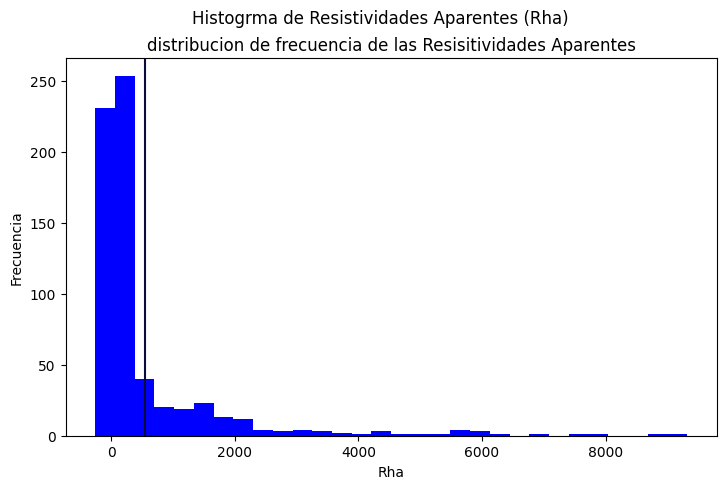
\includegraphics[width=0.9\linewidth]{imagenes/Histograma_Rha}
	\caption[Figura]{Histograma generado a partir de los datos de Rha, densidad de probabilidad, distribución de las resistividades}
	\label{fig:histogramarha}
\end{figure}



\subsection{Correlación y Selección de Variables}\label{subsec5}


\subsection{Entrenamiento de Modelo}\label{subsec6}

\section{Resultados}\label{sec4}


\section{Discusión}\label{sec5}

Discussions

\section{Conclusión}\label{sec6}

Conclusions




\bmhead{Agradecimientos}

Acknowledgments are not compulsory. Where included they should be brief. Grant or contribution numbers may be acknowledged.

Please refer to Journal-level guidance for any specific requirements.



\begin{appendices}

\section{Section title of first appendix}\label{secA1}

An appendix contains supplementary information that is not an essential part of the text itself but which may be helpful in providing a more comprehensive understanding of the research problem or it is information that is too cumbersome to be included in the body of the paper.

%%=============================================%%
%% For submissions to Nature Portfolio Journals %%
%% please use the heading ``Extended Data''.   %%
%%=============================================%%

%%=============================================================%%
%% Sample for another appendix section			       %%
%%=============================================================%%

%% \section{Example of another appendix section}\label{secA2}%
%% Appendices may be used for helpful, supporting or essential material that would otherwise 
%% clutter, break up or be distracting to the text. Appendices can consist of sections, figures, 
%% tables and equations etc.

\end{appendices}


	\begin{thebibliography}{X}\label{sec7}
	
	\bibitem{Joaquin2023} \textsc{Joaquín Amat, Rodrigo}
	\textit{Machine learning con Python y Scikit-learn}, available under a Attribution 4.0 International (CC BY 4.0), Fecha de consulta: 26/03/23,\\
	Url: https://www.cienciadedatos.net/documentos/py06\_machine\_learning\_\\
	python\_scikitlearn.html.\\
	
	\bibitem{Cesano2000} \textsc{Cesano, D., Olofsson, B.} y \textsc{Bagtzoglou, A. C.}(2000),
	\textit{Parameters regulating groundwater inflows into hard rock tunnels—a statistical study of the Bolmen tunnel in southern Sweden}, Tunnelling and Underground Space Technology, 15(2), 153-165.
	
	\bibitem{Parsekian2017} \textsc{Parsekian, A. D., Claes, N., Singha, K., Minsley, B. J., Carr, B., Voytek, E.} y \textsc{Flinchum, B.}(2017),
	\textit{Comparing measurement response and inverted results of electrical resistivity tomography instruments}, Journal of Environmental and Engineering Geophysics, 22(3), 249-266.
	
	%	\bibitem{Dan} \textsc{Dantzig, G.B.} y \textsc{P. Wolfe},
	%	<<Decomposition principle for linear programs>>,
	%	\textit{Operations Research}, \textbf{8}, págs. 101--111, 1960.
	
	\bibitem{Gutierrez2013} \textsc{Gutierrez, R. B.,} y \textsc{i Cintas, P. G.}(2013),
	\textit{El histograma como un instrumento para la comprensión de las funciones de densidad de probabilidad.}, robabilidad Condicionada: Revista de didáctica de la Estadística, 22(3), P, (2), 229-235.
	
	 
	
	
	\end{thebibliography}



\end{document}
